\documentclass[letterpaper,11pt]{article}
\usepackage{tabularx} % extra features for tabular environment
\usepackage{amsmath}  % improve math presentation
\usepackage{graphicx} % takes care of graphic including machinery
\usepackage[margin=0.75in,letterpaper]{geometry} % decreases margins
\usepackage{cite} % takes care of citations
\usepackage[final]{hyperref} % adds hyper links inside the generated pdf file
\hypersetup{
	colorlinks=true,       % false: boxed links; true: colored links
	linkcolor=black,        % color of internal links
	citecolor=blue,        % color of links to bibliography
	filecolor=magenta,     % color of file links
	urlcolor=blue         
}
\usepackage{blindtext}

%%%%%%%%%%%%%%%%%%%%%%%%%%%%%%%%%%%%%%%%%%%%%%%%%%%%%%%%%%%%%%%%%%%%%%%%%%%%%%%%%%%%%%%

% MY PACKAGES

% smart par skip
\usepackage{parskip}

% used to create cute quote 
\usepackage{csquotes}

% fix annoying positioning
\usepackage{float}

% cute tables
\usepackage{booktabs}

% testo intorno a figure
\usepackage{wrapfig, blindtext}

% used to highlight stuff
\usepackage{color,soul}

% MORE MATH
\usepackage{amsfonts}
\usepackage{amsmath}
\usepackage{amssymb}
\usepackage{mathrsfs}

% line breaks in cells
\usepackage{makecell, boldline}

% fix urls in bib
\usepackage{etoolbox}
\appto\UrlBreaks{\do\-}

%%%%%%%%%%%%%%%%%%%%%%%%%%%%%%%%%%%%%%%%%%%%%%%%%%%%%%%%%%%%%%%%%%%%%%%%%%%%%%%%%%%%%%%

% CUSTOM SETTINGS

\setlength\parindent{0pt}

% IMAGES SHORTCUT
\graphicspath{ {./images/} }

% INLINE CODE TEXT
\definecolor{codegray}{gray}{0.9}
\newcommand{\code}[1]{\colorbox{codegray}{\texttt{#1}}}

% CUSTOM LINESPREAD
\linespread{1.05}

% FAST CENTERED IMAGE
\newcommand{\imgc}[3]{\begin{figure}[H] 
  \centering
  \includegraphics[width=#1]{#2}
  \caption{#3}
\end{figure}}

% FIX CAPTION SPACE
\usepackage[font=small,skip=0.25cm]{caption}
\setlength{\belowcaptionskip}{-0.25cm}

% custom line width
\makeatletter
\def\thickhline{%
  \noalign{\ifnum0=`}\fi\hrule \@height \thickarrayrulewidth \futurelet
   \reserved@a\@xthickhline}
\def\@xthickhline{\ifx\reserved@a\thickhline
               \vskip\doublerulesep
               \vskip-\thickarrayrulewidth
             \fi
      \ifnum0=`{\fi}}
\makeatother

% custom citations
\usepackage{cite}

% images wrappers

\usepackage{graphicx}
\usepackage{wrapfig}

% page background color
\usepackage{xcolor}
\definecolor{resblack}{RGB}{30,30,30}
\definecolor{ivory}{RGB}{244,239,233}

%%%%%%%%%%%%%%%%%%%%%%%%%%%%%%%%%%%%%%%%%%%%%%%%%%%%%%%%%%%%%%%%%%%%%%%%%%%%%%%%%%%%%%%

% CUSTOM PYTHON CODE

\usepackage{listings}
\usepackage{xcolor}

\definecolor{codegreen}{rgb}{0,0.6,0}
\definecolor{codegray}{rgb}{0.5,0.5,0.5}
\definecolor{codepurple}{rgb}{0.58,0,0.82}
\definecolor{backcolour}{rgb}{0.95,0.95,0.92}

\lstdefinestyle{mystyle}{
    backgroundcolor=\color{backcolour},   
    commentstyle=\color{codegreen},
    keywordstyle=\color{magenta},
    numberstyle=\tiny\color{codegray},
    stringstyle=\color{codepurple},
    basicstyle=\ttfamily\footnotesize,
    breakatwhitespace=false,         
    breaklines=true,                 
    captionpos=b,                    
    keepspaces=true,                 
    numbers=left,                    
    numbersep=5pt,                  
    showspaces=false,                
    showstringspaces=false,
    showtabs=false,                  
    tabsize=2
}

\lstset{style=mystyle}

%%%%%%%%%%%%%%%%%%%%%%%%%%%%%%%%%%%%%%%%%%%%%%%%%%%%%%%%%%%%%%%%%%%%%%%%%%%%%%%%%%%%%%%

\begin{document}

\pagecolor{ivory}

\title{\textbf{Network and Practical}}
\author{\textbf{Introduction to ML for Natural Language Processing}\\ \\ Daniele Passabì [221229], Data Science\\}

\date{\textit{\\Multi-class Classification of European Laws in Five Languages\\How do Neural Networks and Statistical Models Behave?}}
\maketitle
\thispagestyle{empty}

\begin{figure}[H] 
  \centering
  
\includegraphics[width=4cm]{logo.png}
\end{figure}

\newpage
\pagecolor{white}
\setcounter{tocdepth}{2}
\tableofcontents
\thispagestyle{empty}

\newpage
\clearpage
\pagenumbering{arabic}

%%%%%%%%%%%%%%%%%%%%%%%%%%%%%%%%%%%%%%%%%%%%%%%%%%%%%%%%%%%%%%%%%%%%%%%%%%%%%%%%%%%%%%%
% START HERE
%%%%%%%%%%%%%%%%%%%%%%%%%%%%%%%%%%%%%%%%%%%%%%%%%%%%%%%%%%%%%%%%%%%%%%%%%%%%%%%%%%%%%%%

%%%%%%%%%%%%%%%%
% INTRODUCTION %
%%%%%%%%%%%%%%%%

\section{Introduction}

Natural Language Processing (NLP) originated in the 1950s as the intersection of
artificial intelligence and linguistics \cite{nadkarni2011natural}. It arose in response to the many challenges presented by natural language.

The ambiguity of human language makes it extremely difficult to write software that accurately determines the meaning of text or speech data. Creating hand-written algorithms and rules that can work on any text is very complex, given the presence of homonyms, homophones, sarcasm, unspoken content, idioms, metaphors, grammar and usage exceptions in virtually any text.

NLP combines computational linguistics with statistical models and machine learning in order to successfully process human language in the form of text or speech, understanding its meaning in ways that traditional algorithms are unable to do \cite{IBM_NLP}.

Natural Language Processing is used to solve a wide range of tasks: in this work we are interested in the one of multi-class text classification. Furthermore, our attention will be drawn to a particularly problematic aspect of the NLP field: the fact that most algorithms are designed and implemented for only 7 of the more than 7000 languages spoken in the world. These are English, Chinese, Urdu, Farsi, Arabic, French, and Spanish \cite{TDS_NLP}.

Our objective aims to test whether different languages can influence architectures such as neural networks or statistical models. To this end, we used a dataset containing 65000 European laws, officially translated into several languages, on which we were able to compare the behaviour of various architectures, both with regard to fine-tuning and their performance.

The project code is public and available on \href{https://github.com/DanielePassabi/Uni_NLP2022_Exam}{Github}.
 


%%%%%%%%
% DATA %
%%%%%%%%
\section{Data}

The chosen dataset is called \textit{MultiEURLEX} and is available on \href{https://huggingface.co/datasets/multi_eurlex}{HuggingFace}. It comprises 65000 European laws officially translated into 23 languages. 

Of these available languages, five were selected, based on their adoption at European level:

\begin{itemize}
  \itemsep-0.43em
  \item \textit{English}, with 51\% EU speakers
  \item \textit{German}, with 32\% EU speakers
  \item \textit{Italian}, with 16\% EU speakers
  \item \textit{Polish}, with 9\% EU speakers
  \item \textit{Swedish}, with 3\% EU speakers
\end{itemize}


For each text in the dataset, there are one or more annotated labels indicating the typology of the law. However, as can be understood by reading the paper on the dataset, these annotations are \textit{granular} \cite{Chalkidis2021MultiEURLEXA}. This allowed us to keep only the first level of labels, transforming the problem from a multi-label task to a multi-class one. This operation both simplified the classification and facilitated the evaluation of the architectures results.

This resulted in 21 different classes being initially present, shown in Figure \ref{fig:original_classes} together with the number of occurrences (texts) available for each of them.

A preliminary analysis of the data, however, revealed that each law averaged around 1000 words, with slight fluctuations depending on the considered language. Being aware that this factor would be computationally burdensome during the training phase of the models, it was decided to choose 2000 random laws from each of the three classes with the most observations, i.e. class 2, 3 and 18.

\begin{figure}[H]
  \centering
  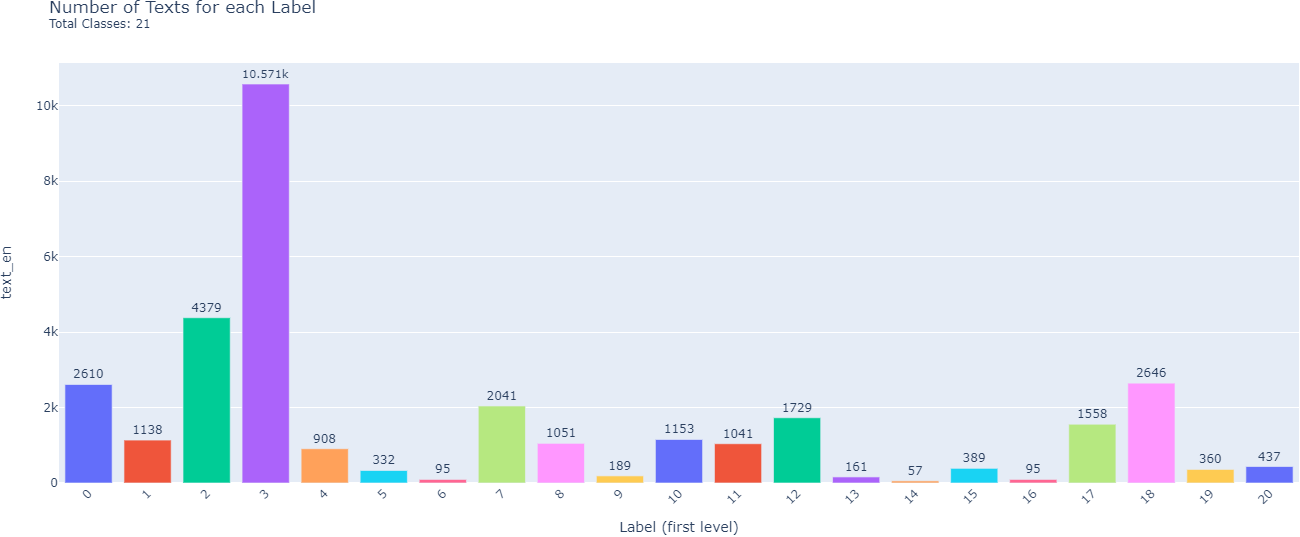
\includegraphics[width=\textwidth]{data_original_classes.png}
  \caption{MultiEURLEX Dataset - Distribution of Classes and Texts Occurrences}
  \label{fig:original_classes}
\end{figure}



Ultimately, the final dataset consists of 6000 laws, officially translated into 5 languages and belonging to 3 distinct classes.

%%%%%%%%%%%%%%%%%
% ARCHITECTURES %
%%%%%%%%%%%%%%%%%
\section{Architectures}
\label{sec:architectures}

In order to test the impact of different languages, various architectures were chosen, belonging both to the world of neural networks and statistics.

For reasons of limited space, one architecture per typology is presented in detail: for neural networks, the functioning of an LSTM is explained in depth; for statistical models, the Linear Support Vector Classifier is illustrated. Nevertheless, the CNN architecture is briefly introduced.

\subsection{Long Short Term Memory}

The Long Short Term Memory (LSTM) is a kind of recurrent neural network (RNN). RNNs are a type of networks particularly suited to the use of sequential data, or time series. 

A distinguishing characteristic from the traditional neural networks is their capacity to have a \textit{memory}: they use information obtained from previous inputs to modify their behaviour on the current input and output. They keep the information of the former inputs in memory for an unspecified time, which depends on the weight of the network nodes and the specific data. Recurrent neural networks do not assume that input and output are independent, as traditional networks do, but make their output depend on the previous elements in the sequence. Figure \ref{figure:fnn_vs_rnn} shows the typical structure of a feedforward neural network on the left, and that of a recurrent neural network on the right.

\vspace{0.25cm}
\begin{figure}[H]
  \centering
  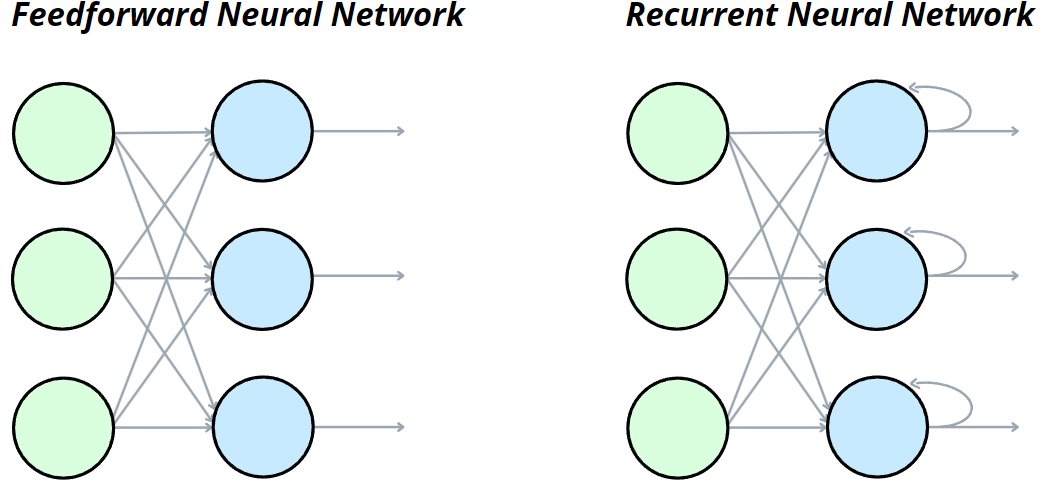
\includegraphics[width=6.9cm]{feedforward_vs_recurrent_nn.png}
  \caption{Structure of Feedforward and Recurrent Neural Networks}
  \label{figure:fnn_vs_rnn}
\end{figure}

Recurrent neural networks use an algorithm of \textit{backpropagation through time} to determine gradients. Backpropagation is at the basis of neural networks training, making possible the fine tuning of their weights, based on the results obtained in the previous epochs. The \textit{gradient} refers to the derivative of a function that has more than one input variable; it measures the change in all the weights of the network with respect to the change error. 

During this operation, recurrent neural networks tend to encounter two types of problems, both arising from the size of the gradient:
\begin{itemize}
  \item \textit{Vanishing Gradients}
  
  In some circumstances, the gradient is very small and continues to decrease until it becomes extremely close to 0. When this happens, the model stops learning, as its weights are no longer updated.

  \item \textit{Exploding Gradients}
  
  Conversely, the gradient can become extremely large, altering the network weights unreasonably. This causes the model to become unstable and consequently underperforming.
\end{itemize}

Long Short Term Memory networks were conceived in response to the problems of vanishing and exploding gradient, proposing a possible solution to these issues \cite{LSTM_gentle_intro}. A clear description of the inner workings of LSTMs can be found in the paper by Graves et al. \cite{Graves2005FramewisePC} where it is detailed that:

\begin{quote}
  \textit{``An LSTM layer consists of a set of recurrently connected blocks, known as memory blocks. These blocks can be thought of a differentiable version of the memory chips in a digital computer. Each one contains one or more recurrently connected memory cells and three multiplicative units - the input, output and forget gates - that provide continuous analogues of write, read and reset operations for the cells.''}
\end{quote}

In order, what happens is:
\begin{enumerate}
  \item The cell input is multiplied by the activation of the input gate;
  \item The model output is multiplied by the output gate activation;
  \item Finally, the previous cell values are multiplied by the forget gate values. 
\end{enumerate}

The network is capable of interacting with its cells exclusively through the use of gates.  

LSTMs achieve remarkably high performance on major and complex tasks; these include language modelling, speech recognition and machine translation \cite{Zaremba2014RecurrentNN}.


\subsection{Convolutional Neural Network}

Convolutional neural networks (CNN) are one of the most renowned algorithms of deep learning. Under the deep learning category fall all those artificial neural networks that have more than one layer (and are thus called multi-layer architectures).

The layers of CNNs are usually the following: \textit{Convolutional Layer}, \textit{Non-Linearity Layer}, \textit{Pooling Layer} and \textit{Fully Connected Layer}. We will explain part of these layers in subsection \ref{subsec:implementation}, concerning the implementation of our architectures.

The models that use convolutional neural networks have shown over the years that they are able to achieve state of the art results in many Machine Learning problems. CNNs perform particularly well in image classification and computer vision tasks, but they have also proven powerful in problems of Natural Language Processing \cite{Albawi2017UnderstandingOA}.

\subsection{Linear Support Vector Classifier}

In order to fully understand the idea behind the Linear Support Vector Classifier, it is first necessary to introduce some concepts that form its foundation.

First, let us introduce the notion of \textit{hyperplane}. Intuitively, it is possible to think of the hyperplane as something that divides space into two sides, where it is straightforward to determine in which of the two sides a point is located. An example of hyperplane in two-dimensional space can be observed in Figure \ref{figure:hyperplane_2d}.

\begin{wrapfigure}{R}{0.35\textwidth}
  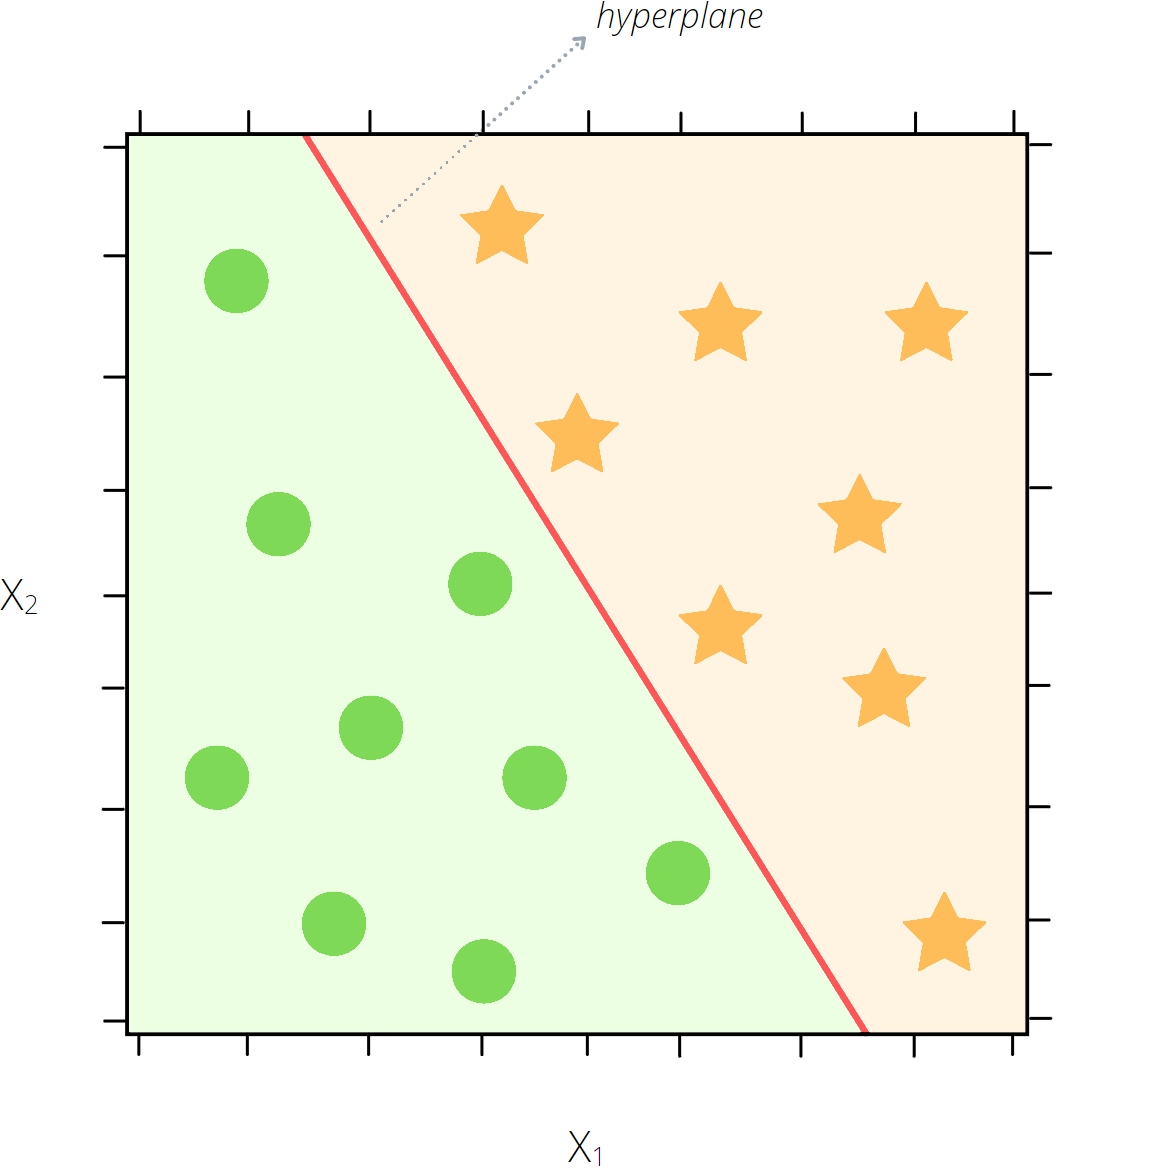
\includegraphics[width=6cm]{hyperplane_example.png}
  \caption{Hyperplane in 2D case}
  \label{figure:hyperplane_2d}

  \vspace{1.15cm}

  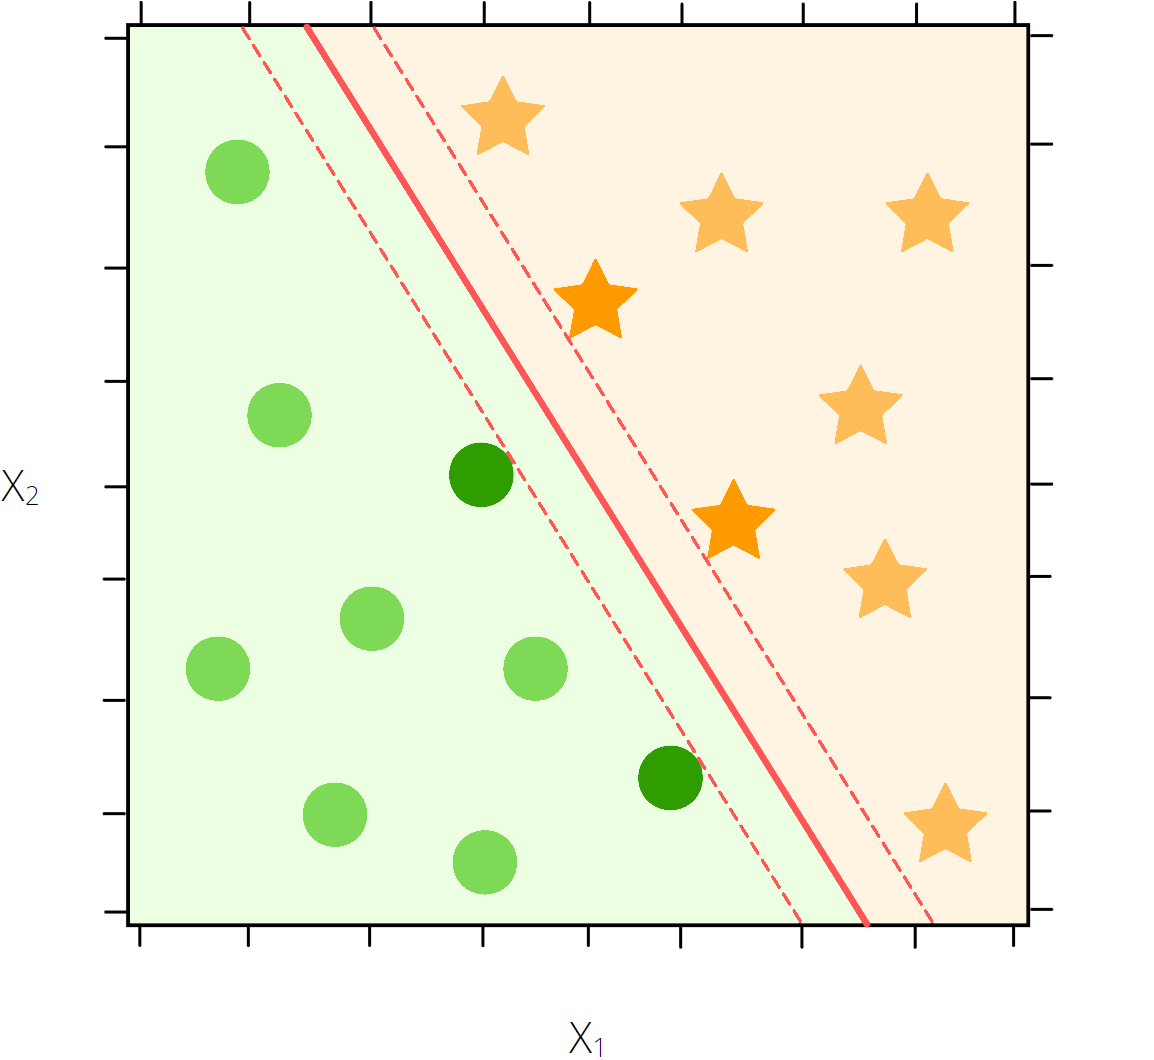
\includegraphics[width=6cm]{max_hyperplane.png}
  \caption{Maximum Margin Hyperplane and Support Vectors (highlighted points)}
  \label{figure:max_margin_classifier}
\end{wrapfigure}


The visualisation also suggests how a hyperplane can be used to classify different observations. Let's suppose that the points in the figure represent the training set, i.e. the data initially available for training a model. It is then possible to construct a classifier in a very straightforward way: new points will be classified into \textit{green} or \textit{yellow observations} according to their position in space, given by $X_1$ and $X_2$.

Depending on how close the new observation is to the hyperplane it is also possible to have a certain degree of confidence in the correctness of the prediction. For points close to the separating hyperplane we are less certain about their class than for those further away.

% \begin{wrapfigure}{R}{0.35\textwidth}
%   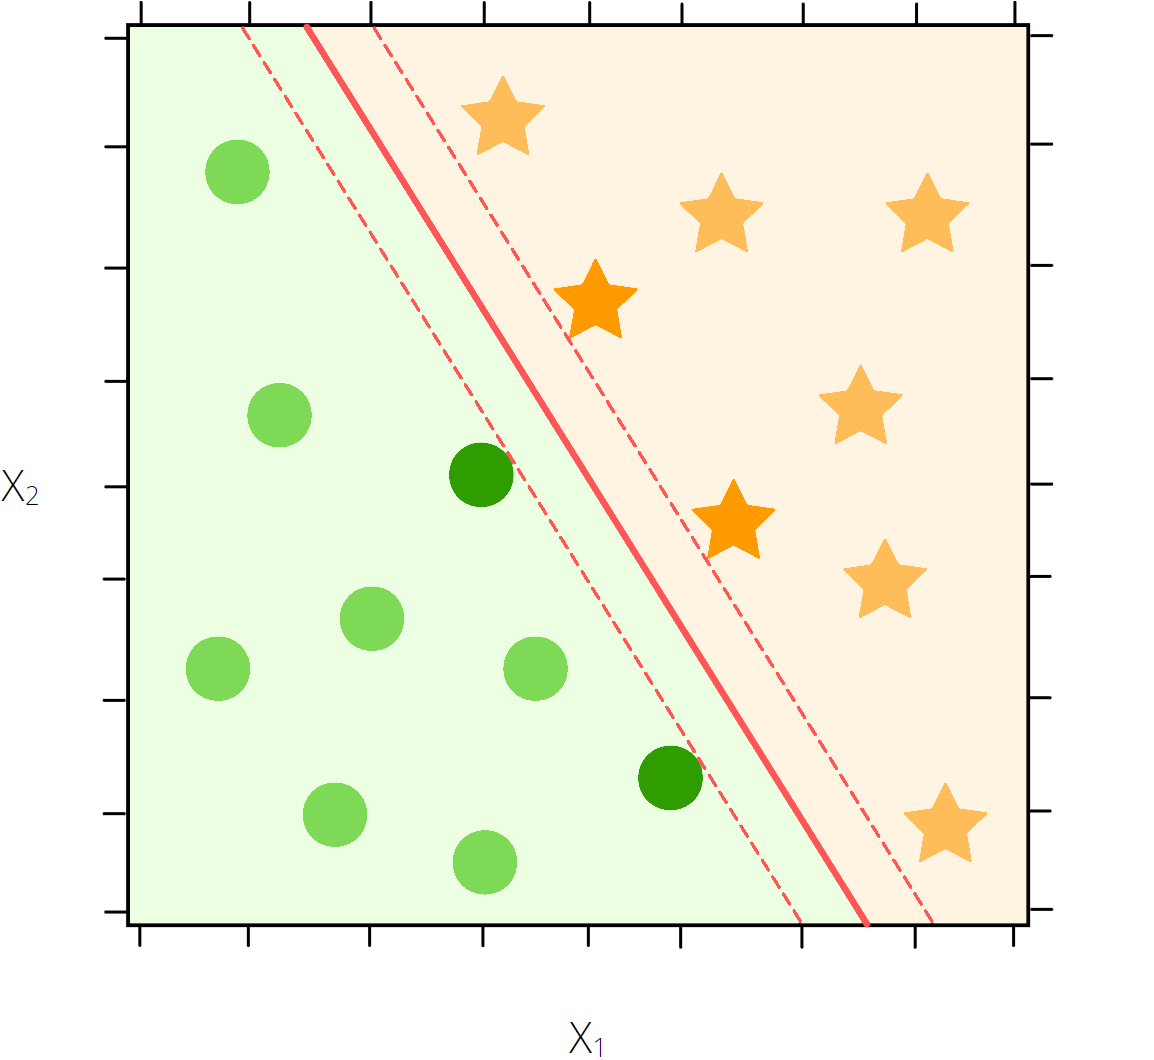
\includegraphics[width=6cm]{max_hyperplane.png}
%   \caption{Maximum Margin Hyperplane and Support Vectors (highlighted points)}
%   \label{figure:max_margin_classifier}
% \end{wrapfigure}

There can exist an infinite number of different hyperplanes able to separate the green observations from the yellow ones. For this reason it is necessary to decide how to choose the \textit{best} hyperplane. An appropriate choice is to use the \textit{maximal margin hyperplane}, which is the hyperplane most distant from the training observations. It depends entirely on the so-called \textit{support vectors}, i.e. the points closest to it that influence its position and orientation. See Figure \ref{figure:max_margin_classifier} for an example.

Until now we have discussed a binary case in which the two classes were linearly separable. In the event that they are not, as it happens in many real world cases, it is no longer possible to find the maximum margin hyperplane. Even if it were feasible to find it, using it is not always the best solution: trying to perfectly separate the observations of the two classes makes the maximum margin hyperplane very sensitive to individual observations. It may be a better solution, in many cases, to consider a hyperplane that does not perfectly separate the training observations, but that allows to obtain a higher robustness regarding the individual observations and that correctly classifies most of the training observations.

This is indeed the objective of the Linear Support Vector Classifier. The model purposely allows the misclassification of certain observations, in order to correctly classify as many points as possible, while maximising the width of the margin.

Since in our specific case we are working with 3 classes, we are not in a binary classification scenario. We have therefore extended the binary approach to a multiclass approach using the scheme \textit{One-VS-Rest}. It is a heuristic that allows us to split our multiclass dataset into multiple binary classification problems.


%%%%%%%%%%%%%%%%%%%%%%
% EXPERIMENTAL SETUP %
%%%%%%%%%%%%%%%%%%%%%%
\newpage
\section{Experimental Setup}

\subsection{Data Cleaning and Preprocessing}

The majority of data is prone to the presence of errors and noise. This is particularly true in the field of Natural Language Processing. Therefore, textual data must be subjected to pre-processing procedures before being given to the models. 

The first critical step is data cleaning. In addition to the usual procedures such as removing duplicates, missing data, etc., when working with textual data, one often has to deal with texts that contain spelling mistakes, the use of jargon and symbols that are not useful for learning models. In our specific case, using a dataset of officially translated European laws, we do not have to worry about these issues. 

Furthermore, texts always contain \textit{stopwords}, commonly used terms that do not provide information, and which it is common practice to remove. However, these removal procedures use lists of words considered to be stopwords, but there are no universal rules. In order not to give any advantages to the most frequently used languages, such as English and German, we have decided not to remove them from the texts. Furthermore, working with recurrent neural networks like LSTMs, stopwords could increase the contextual sense of the networks and, contrary to what usually happens in other tasks, improve the performance of the models.

Another technique used when working with texts and natural language is to apply stemming or lemmatization procedures. These are described below.
\begin{itemize}
  \item \textit{Stemming}
  
  As can be found in the article \textit{Development of a stemming algorithm} \cite{lovins1968development}:
  \begin{quote}
    \textit{``A stemming algorithm is a computational procedure which reduces all words with the same root (or, if prefixes are left untouched, the same stem) to a common form, usually by stripping each word of its derivational and inflectional suffixes.''}
  \end{quote}
  
    \item \textit{Lemmatization}
  
  It is a procedure that removes inflectional endings and returns the base or dictionary form of a word.

  This technique ensures that similar words are reduced to the same word, which often leads to higher performance in models \cite{balakrishnan2014stemming}. 

\end{itemize}

However, the same logic of stopwords applies to {stemming} and {lemmatization} procedures, which are therefore not applied to texts.

It is only fair to mention that the initial dataset has a very high quality: it was thus only necessary to lowercase all words, remove symbols and non-unicode characters, in order to ensure the proper functioning of future architectures.

\subsection{Feature Extraction}
\label{subsec:feature_extr}

Feature extraction describes the process of transforming raw data into numerical features that can be processed while retaining the information in the original dataset.

There are several ways of extracting information from data, and they change depending on the type of input that is being handled. In the context of this work, the primary focus is on the extraction of features from natural language. The procedures employed are outlined below.

\subsubsection*{Feature Extraction for Neural Networks}

With regard to the creation of features for the neural networks used, namely long short term memory and convolutional neural network, we performed the following procedures:

\begin{itemize}
  \item \textit{Tokenization}
  
  It involves breaking up a raw text into smaller pieces. In our case, we break down each law text into words, the tokens. 

  \item \textit{Count Token Occurrences}
  
  We count the number of occurrences of each token (word) in our five corpuses.

  This is where we noticed the first difference between the languages: the number of different unique words used changes considerably, as can be seen in the Table \ref{table:tot_words_for_corpuses}. The German language, for example, uses almost three times as many words as English to write the same laws.

 \begin{table}[H]
    \centering
    \begin{tabular}{@{}rl@{}}
    \toprule
    \multicolumn{1}{c}{\textbf{Language}} & \textbf{Unique Words} \\ \midrule
    English                               & 31454                 \\
    German                                & 87084                 \\
    Italian                               & 44570                 \\
    Polish                                & 74691                 \\
    Swedish                               & 79973                 \\ \bottomrule
    \end{tabular}
    \caption{Total number of unique words in each language corpus}
    \label{table:tot_words_for_corpuses}
    \end{table}


  \item \textit{Removal of Uncommon Words}
  
  The number of different words in the texts is very high. This factor would certainly negatively affect the performance of the architectures or, at the very least, make training times extremely long. 
  
  In order to avoid these possible drawbacks, all words that did not appear in the corpus at least 100 times were removed. Table \ref{table:tot_words_for_corpuses_only_common} shows the number of words left for each language after this operation.
  
  \begin{table}[H]
    \centering
    \begin{tabular}{@{}rl@{}}
    \toprule
    \multicolumn{1}{c}{\textbf{Language}} & \textbf{Unique Words} \\ \midrule
    English                               & 3506                   \\
    German                                & 4216                   \\
    Italian                               & 4180                   \\
    Polish                                & 5255                   \\
    Swedish                               & 4010                   \\ \bottomrule
    \end{tabular}
    \caption{Total number of unique words in each language corpus that appears at least 100 times}
    \label{table:tot_words_for_corpuses_only_common}
    \end{table}

  After this adjustment, the disparity between languages in the number of different words has softened, but is still present.

  \item \textit{Encoding}
  
  In this last step, we created a mapping between vocabulary and index, in order to use it in the encoding of the texts. Here, we had to set a maximum token number for each text. Since the average number of words per law is about 1000, we used this value as an upper limit.


\end{itemize}


\subsubsection*{Feature Extraction for Linear Support Vector Classifier}

Text Vectorization is a technique that consists of transforming textual data into numerical vectors that can be understood by machine learning architectures.

One of the most widely adopted techniques for text vectorization is \textit{Term Frequency - Inverse Document Frequency} (TF-IDF), a statistical measure that assesses how relevant a word is to a document in a collection of documents.

In the case of laws classification, the text of each law represents one document.

The TF-IDF score for a word is obtained by multiplying the two metrics that compose the algorithm:

\begin{itemize}
  \item \textit{Term Frequency (TF)}
  
  In its simplest form, it refers to the number of times a word appears in a document.

  \item \textit{Inverse Document Frequency}
  
  It refers to how common a word is in the entire set of sentences. The more frequent a word is, the closer its value is to 0.

  It is possible to calculate the IDF of a word by obtaining the total number of documents, dividing it by the number of documents containing that given word and computing the logarithm.
\end{itemize}

Multiplying these two values makes it possible to obtain the TF-IDF of a word in a document. The higher the value, the greater the relevance of the word within a document.

The TF-IDF is an efficient solution to the problem of \textit{stopwords}: since they are frequent words in all documents, they have a value very close to zero and do not become influential for the models. The intriguing aspect is that this logic should be applicable to any language.

If a word is repeated many times within the same document, on the contrary, it might indicate its importance. The algorithm is able to detect these subtleties and is a particularly effective way of preparing the input for future architectures.


\subsection{Implementing the Architectures}
\label{subsec:implementation}

A brief description of the implementation of the architectures presented in Section \ref{sec:architectures} follows. In the case of neural networks, we focus on the employed layers.

\subsubsection*{Long Short Term Memory}

The architecture was implemented using the \verb|PyTorch| framework. 
In the development of the network, the following layers were used:

\begin{itemize}
  \item \textit{Embedding Layer}
  
  \vspace{-0.6mm}
  
  This layer is often used to store and retrieve word embeddings using indexes. The input of the module is a list of indexes and the output is the corresponding word embedding \cite{pytorch_embedding}.
  \item \textit{LSTM Layer}
  
  \vspace{-0.6mm}

  As one can easily deduce from its name, this module is the heart of the network. It applies a multi-layer long short-term memory to an input sequence \cite{pytorch_lstm}.
  \item \textit{Linear Layer}
  
  \vspace{-0.6mm}
  
  Its purpose is to apply a linear transformation to the input data \cite{pytorch_linear}.
  \item \textit{Dropout Layer}
  
  During the training phase, some elements of the input tensor are zeroed with probability $p$, using samples of a Bernoulli distribution.

  This technique has proven to be effective in regularising and preventing co-adaptation of neurons \cite{pytorch_dropout}, which refers to those cases in which some neurons are highly dependent on others.
\end{itemize}


% USA QUESTO CODICE
% input_names = ['Law Text']
% output_names = ['Law Label']
% torch.onnx.export(model, batch.text, 'rnn.onnx', input_names=input_names, output_names=output_names

\subsubsection*{Convolutional Neural Network}

This architecture, like the illustrated one above, has also been implemented using the \verb|PyTorch| framework. Note: some layers are the same as those employed for the LSTM and will thus not be explained again.

\begin{itemize}
  \item \textit{Embedding Layer}
  \item \textit{Convolutional 1D Layer}
  
  Convolutional layers are one of the main building blocks used in convolutional neural networks. The term \textit{convolution} refers to the application of a filter to an input, which then produces an activation. A repeated application of the same filter to an input produces an activation map, also called a feature map, which indicates the position and strength of a detected feature in an input.

  It is a linear operation involving the multiplication of a set of weights with the input, a common operation in neural networks \cite{CNN_how}.
  \item \textit{Max Pooling 1D Layer}
  
  Pooling layers make it easy to down-sample feature maps. They summarise the presence of features in patches of the feature map. 
  
  One of the most widely used pooling levels is max pooling, partly due to its high performance. In this instance, the pooling operation calculates the maximum value in each patch of each feature map \cite{MaxPool_how}.
  \item \textit{Linear Layer}
  \item \textit{Dropout Layer}
\end{itemize}





\subsubsection*{Linear Support Vector Classifier}

This architecture was developed using the \verb|scikit-learn| framework. Since it is a more high-level library than \verb|Pytorch|, the implementation was simpler and more straightforward. Most of the work consisted in obtaining suitable features for the model, which was performed via the TF-IDF algorithm presented in subsection \ref{subsec:feature_extr}.

\subsection{Training Regime}
\label{subsec:fine_tuning}

During the course of the project, particular emphasis was placed on fine-tuning the models. A detailed explanation of what was performed for each architecture follows.

\subsubsection*{Dataset Splits}

Prior to proceeding with the model training phase, each dataset was divided upstream into three sets: 
\begin{itemize}
  \itemsep-0.42em
  \item \textit{training set} (3840 texts)
  \item \textit{validation set} (960 texts)
  \item \textit{test set} (1200 texts)
\end{itemize}

\subsubsection*{Saving the Best Model}

\underline{\textit{Neural Networks}} During each epoch the models were trained on the training set and validated on the validation one. As loss we have opted for \textit{cross entropy}, which is considered suitable for cases of multiclass classification, both when working with statistical models and NNs \cite{cross_entropy}.

We implemented an automatic mechanism capable of saving the model weights of the best epoch based on the average accuracy of the three classes, along with a dataframe containing the training results. The latter was employed to create data visualizations and better understand what occurred during the training phase, thus making it possibile to observe differences between languages. We will further discuss training results in Section \ref{sec:results}.

\underline{\textit{Statistical Models}} Saving the results of the linear support vector classifiers was straightforward, as we did not have to handle the different epochs. The \textit{squared hinge loss}, proposed as default by the \verb|scikit-learn| framework, was chosen.

\subsubsection*{Long Short Term Memory}

For each of the five available languages, 16 models were trained, i.e. the combination of a grid search performed on the hyperparameters shown in Table \ref{table:LSTM_hyperparameters}.

\begin{table}[H]
  \centering
  \begin{tabular}{@{}rll@{}}
  \toprule
  \multicolumn{1}{c}{\textbf{Hyperparameter}} & \multicolumn{1}{c}{\textbf{Employed By}} & \textbf{Values Tested} \\ \midrule
  \textit{Embedding Dim}                               & Embedding Layer                          & 1024, 2048          \\
  \textit{Hidden Dim}                                  & LSTM Layer                               & 1024, 2048          \\
  \textit{Dropout Probability}                         & Dropout Layer                            & 0, 0.1              \\
  \textit{Learning Rate}                               & Adam Optimizer                           & 0.0001, 0.001       \\ \bottomrule
\end{tabular}
\caption{Hyperparameters tested for LSTM networks}
\label{table:LSTM_hyperparameters}
\end{table}

Each model was trained for a total of 50 epochs, using a batch size of 64. As a note, we are aware that in order to obtain more robust and reliable results it would have been ideal to increase the number of hyper-parameter values tested, along with the number of epochs. Training times, however, would have risen exponentially. Each complete search grid, which trains 16 models over 50 epochs, takes between 14 and 16 hours on an \textit{RTX 2070 Super} GPU, slightly varying according to the language of the texts.

\subsubsection*{Convolutional Neural Network}

Convolutional neural networks proved to be less computationally demanding than LSTMs. This allowed us to test a higher number of hyperparameter values, with a total of 96 models per language (Table \ref{table:CNN_hyperparameters}).

\begin{table}[H]
  \centering
  \begin{tabular}{@{}rll@{}}
  \toprule
  \multicolumn{1}{c}{\textbf{Hyperparameter}} & \multicolumn{1}{c}{\textbf{Employed By}} & \textbf{Values Tested} \\ \midrule
  \textit{Embedding Dim}                   & Embedding Layer                          & 1024, 2048             \\
  \textit{Kernel Size}                   & CNN Layer, Max Pooling Layer             & 3, 5, 7                \\
  \textit{Stride}                   & CNN Layer, Max Pooling Layer             & 1, 3                   \\
  \textit{Padding}                   & CNN Layer                                & 1, 3                   \\
  \textit{Dropout Probability}                   & Dropout Layer                            & 0, 0.1         \\
  \textit{Learning Rate}                   & Adam Optimizer                           & 0.0001, 0.001                 \\ \bottomrule
  \end{tabular}
  \caption{Hyperparameters tested for Convolutional Neural Networks}
  \label{table:CNN_hyperparameters}
\end{table}


As with the LSTMs, the CNNs were also trained for 50 epochs, using a batch size of 64.

\subsubsection*{Linear Support Vector Classifier}

For this architecture, there are no performance concerns. We therefore trained 7 different models for each language, each with a different value of $C$, the model's only hyperparameter.

$C$ is the parameter responsible for \textit{regularization}, which is inversely proportional to its value. Thus, for high values of $C$ the optimiser will choose a hyperplane with a narrower margin if it correctly classifies all points in the training set. Conversely, a small value of $C$ will cause the optimiser to look for a separating hyperplane with a larger margin, even if this hyperplane incorrectly classifies a greater number of points. 

The values that we tested for the $C$ hyper-parameter are the following: 0.1, 1, 5, 10, 50, 100, 1000.



%%%%%%%%%%%
% RESULTS %
%%%%%%%%%%%
\section{Results}
\label{sec:results}

\subsection{Training Times}

Throughout this project we have always kept track of the training times of the models. We believe that this can provide useful insights regarding the differences that are present due to the languages, as well as those present due to the different architectures. A table of training times is shown in Figure \ref{fig:training_times}.

\begin{figure}[H]
  \centering
  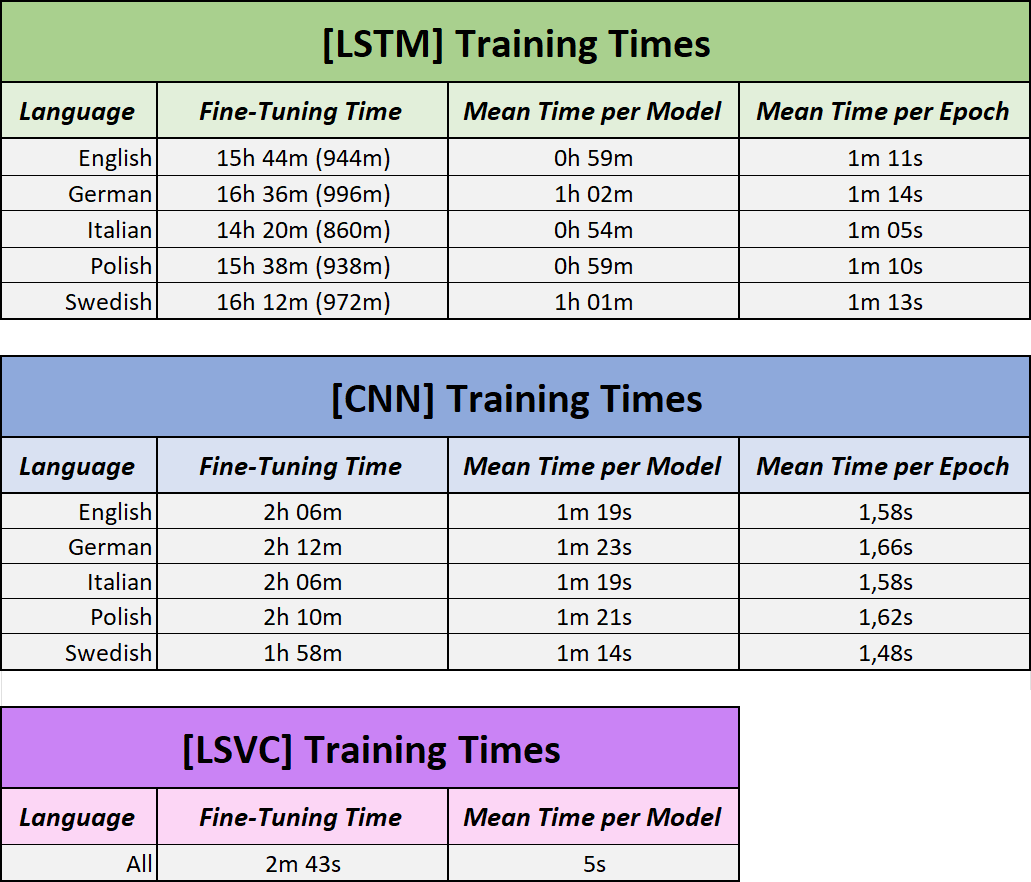
\includegraphics[width=11.28cm]{fine_tuning_times.png}
  \caption{Training Times of the Architectures}
  \label{fig:training_times}
\end{figure}

As can be observed from the illustration, the differences in time due to architectures are significantly greater than those due to the language used. There are, however, considerable time fluctuations in LSTMs when training a model with German or Swedish texts, compared to other languages. 

It is worth noting, however, that although we have attempted to train the models consistently under the same conditions, the computer may autonomously have launched background processes beyond our control that affected training times.

A small technical note: the two neural networks were trained on an \textit{RTX 2070 Super} GPU, while the linear support vector classifiers on an \textit{i7-9700K CPU}.

\subsection{Training Results}

Before discussing the performances of the models, it is of interest to focus on the training phase of the architectures. Figure \ref{fig:hyperparam_epoch_res} shows the best hyperparameters chosen for each architecture of each language, together with the best epoch (in the case of neural networks) and the validation accuracy, obtained as the average of the precision of the three different classes.

It is immediately evident the disparity in the number of hyperparameters present in the neural networks compared to the statistical model, which only has $C$. The higher the number of hyper-parameters, the more difficult it is to conduct an exhaustive fine-tuning, capable of really giving us the best performance the model can offer. 

It is interesting to note that the same values are always chosen for certain hyper-parameters, as in the case of \textit{embedding dimension} and \textit{dropout p} for LSTMs, \textit{stride} for CNNs and \textit{learning rate} for both. Of the seven values of $C$ tested, 1 always proved to be the best for the LSVCs. 

Another aspect we noticed from the empirical results was that even when changing the value of $C$ by several orders of magnitude, the performance of the model varied negatively by a maximum of 2\%. If we consider that, on the other hand, for ``unlucky'' combinations of hyperparameters the performances of the neural networks halves it is possible to realise how robust the linear support vector classifier is.

\begin{figure}[H]
  \centering
  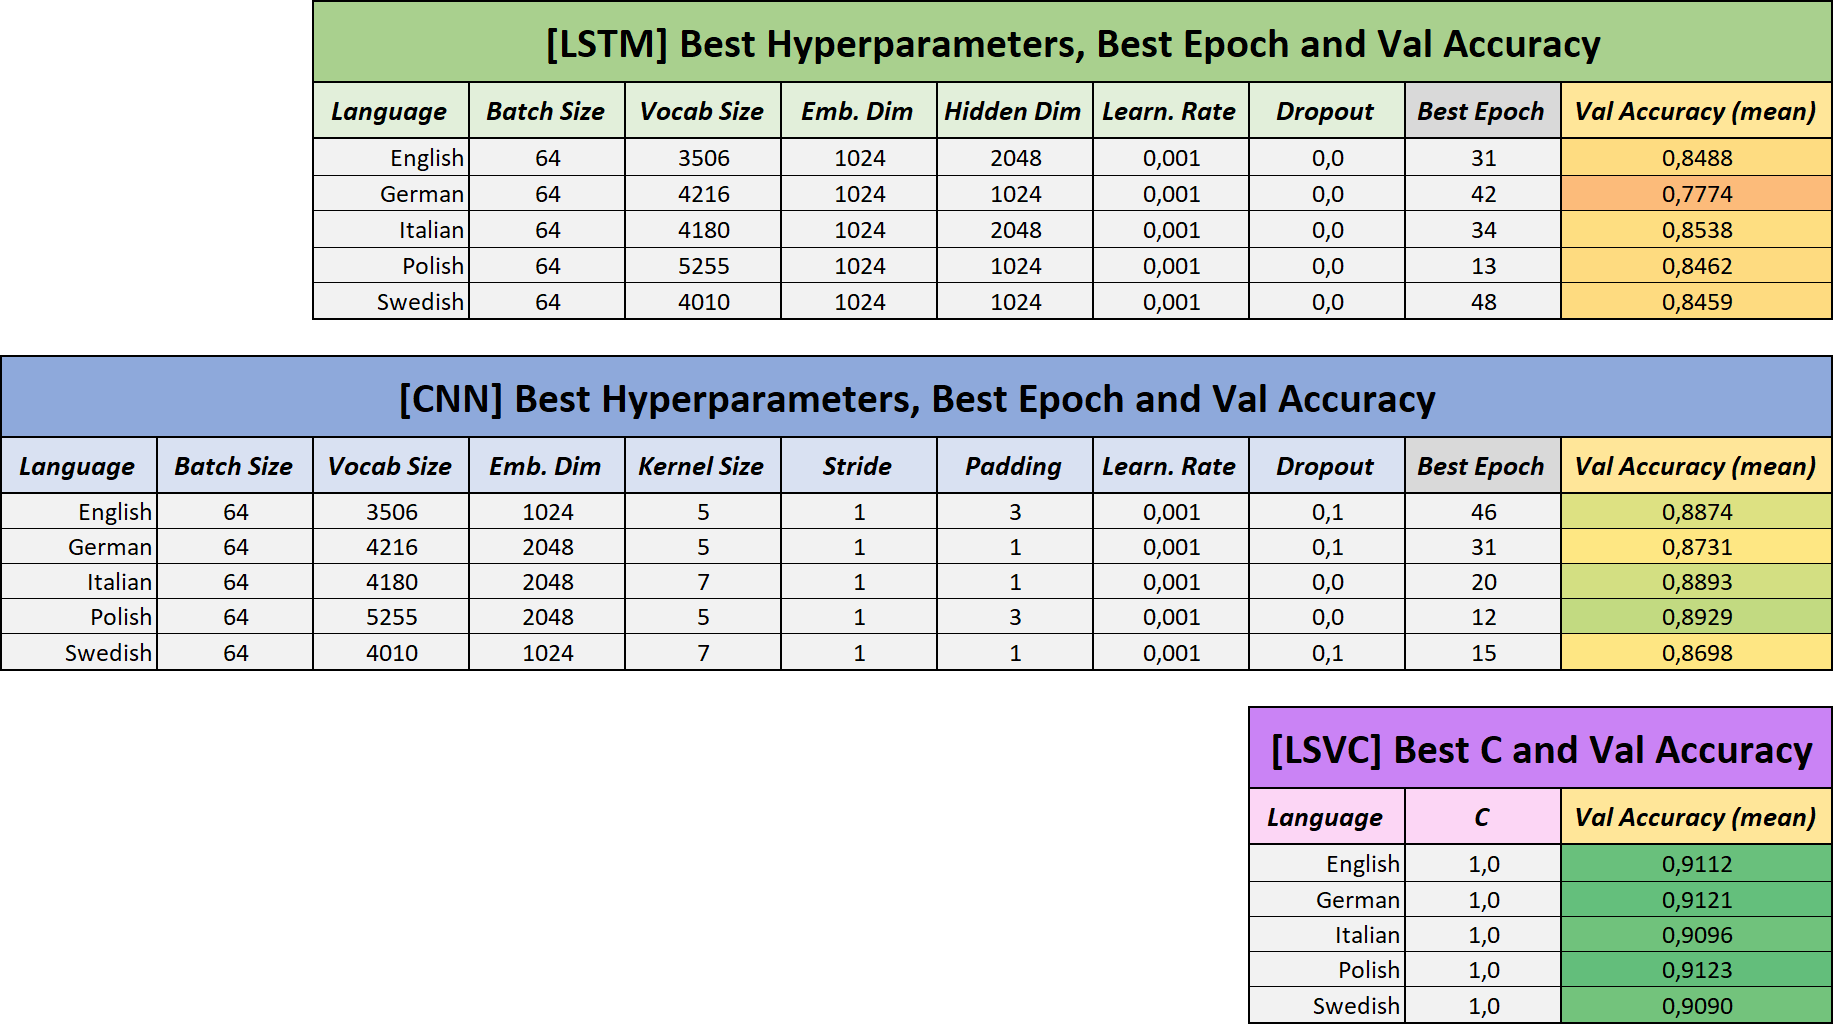
\includegraphics[width=\textwidth]{hyperparam_res.png}
  \caption{Best Hyperparameters, Best Epoch (when available) and Validation Accuracy for each Architecture}
  \label{fig:hyperparam_epoch_res}
\end{figure}


Further interesting insights can be obtained by exploring the two visualisations made for the training phases of the best LSTMs and CNNs, which can be found in Figure \ref{figure:lstm_res} and  \ref{figure:cnn_res}. The first column shows the graphs depicting training and validation loss for each language. The second shows the accuracy of each class as the epochs increase. In both views, the vertical green dashed line indicates the best epoch chosen for that specific model. 

In the case of the LSTMs, one can see how the \textit{training loss} falls, more or less quickly and steadily depending on the language, until it almost reaches 0, a state that is usually associated with overfitting. The \textit{validation loss}, on the other hand, tends to fall and then rise again, assuming its usual elbow shape. It can be seen that in most cases the mean accuracy of the three classes is the highest just before the validation loss starts to rise again.

In the case of CNNs, however, something a little unusual happens. Both the training loss and the validation loss decrease and remain more or less constant in a value between 0.6 and 0.8. This could happen since we only used one convolutional layer in our architecture, which may not be able to fully capture the complexity of the data.

To confirm this thesis, it can be seen in the second column how the performance on the three classes is not very stable and continuously fluctuates. In the LSTMs this does not happen: after a certain number of epochs, the performance of the three classes stabilises (excluding the case of German).  

\subsection{Model Performances}

Figure \ref{fig:results} shows the results obtained from the best architectures for each language on the test set. Colours are used in the visualisation to highlight the differences in the models performances.  

\begin{figure}[H]
  \centering
  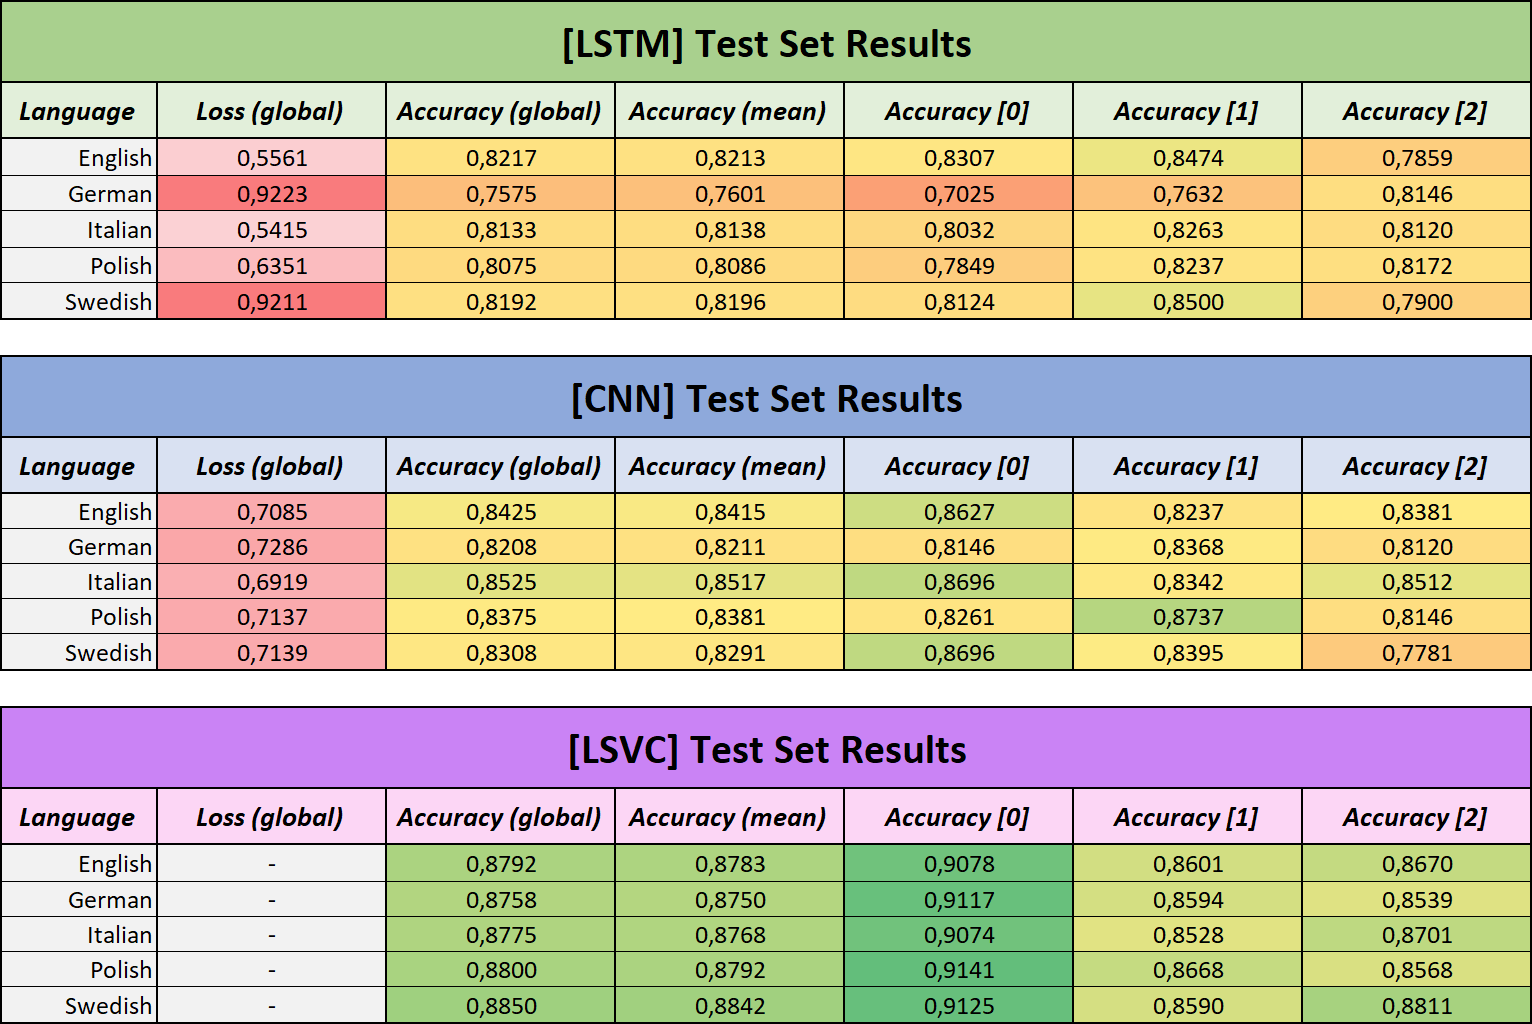
\includegraphics[width=\textwidth]{results.png}
  \caption{Architectures Performances on Test Set}
  \label{fig:results}
\end{figure}

\underline{\textit{LSTM}} LSTM networks have the worst performance despite the highest training times. 

It is interesting to observe how they have the most difficulties classifying German and Swedish texts, which are characterised by a higher loss compared to the other languages and, in the case of German, significantly lower performance. We would certainly need the opinion of an expert linguist, but our assumption is that German has a high number of compound words, which for people immediately acquire a meaning, but for models are completely different from the two words that compose them. Moreover, in some cases the order of the sentence syntagmas changes completely from the usual (example: the verb is placed at the end of the sentence).

It can be observed from the results that, with the exception of one language, class 1 is always the one with slightly higher accuracy.

\underline{\textit{CNN}} Similarly to what happened in the LSTMs, also in the CNNs the lowest performances are achieved by the German and Swedish models, although the difference between them and the performance of the other models is milder. With this type of network, however, the loss values are very close, with no substantial difference dependent on language.

\underline{\textit{LSVC}} It is very interesting to observe how a statistical model that trains in five seconds on any CPU can compete and outperform neural networks that require hours of training on a dedicated GPU. According to the literature, this can happen thanks to TF-IDF, which is very reliable and leads to higher results than the words embedding employed by neural networks \cite{cahyani2021performance}.

The LSVC models do not seem to be influenced by language, and obtain very satisfactory results in all five cases, with little to no difference between them.

It is worth noting that, in contrast to LSTMs, this model predicts class 0 texts with greater ease and consequent accuracy.

%%%%%%%%%%%%%%
% DISCUSSION %
%%%%%%%%%%%%%%
\section{Discussion}

\subsection{About the Results}

During the course of the project, we trained different architectures, belonging to related but different worlds, that of statistics and machine learning.

Our purpose was to understand whether and to what extent texts in different languages would change the training times and performances of the models. We were able to demonstrate the robustness of TF-IDF, which allowed the Linear Support Vector Classifiers to perform very well regardless of the language used.

The analysis also gave us an opportunity to reflect on the fragility of neural networks, which require to be fine-tuned on a high number of parameters and for considerable time in order to have satisfactory results. LSTMs more than CNNs seem to be susceptible to the language they are trained on, presumably since they are sequential models and as such are more influenced by how the sentence is formed, rather than just the words contained within it.

\subsection{Ideas for Expanding the Project}

During the course of the project, choices were made to simplify the task and the training time required by the models. This was mainly done for reasons of limited time and means at our disposal: having only one graphics card available, certain choices proved necessary.

The following is a list of suggestions and ideas through which the project could be expanded, if we had the means to do so.

\begin{itemize}
  \item It would first be interesting to use all the texts of the laws at our disposal and repeat the experiment.
  \item Furthermore, it would also be worthwhile to consider the multi-label task and observe how the architectures behave in different languages.
  \item Having multiple GPUs available, the experiment could be repeated using all 23 languages from the initial dataset.
  \item A further idea is to try applying stopwords removal, lemmatization and/or stemming procedures to texts. The aim here is to see if and how the performance of the models changes and if the procedures favour the most common languages.
  \item With regard to the fine-tuning phase, as already mentioned in the relevant subsection \ref{subsec:fine_tuning}, it would be advisable to extend the range of values used for each hyper-parameter in order to obtain more robust results. 
  
  In this regard, there are some implementable refinements that could save time during the fine-tuning phase:
  \begin{itemize}
    \item An \textit{early stopping} mechanism could be implemented, which interrupts network training if after $n$ epochs the validation loss has not decreased;
    \item One could use more efficient tuning algorithms than the ``brute'' grid search, such as the one proposed by the \verb|Keras| framework \cite{omalley2019kerastuner}. 
  \end{itemize}
\end{itemize}

% RISULTATI TRAINING [2 black pages]

\newpage
\pagecolor{resblack}
\begin{figure}[H]
  \vspace*{-1.75cm}
  \makebox[\linewidth]{
    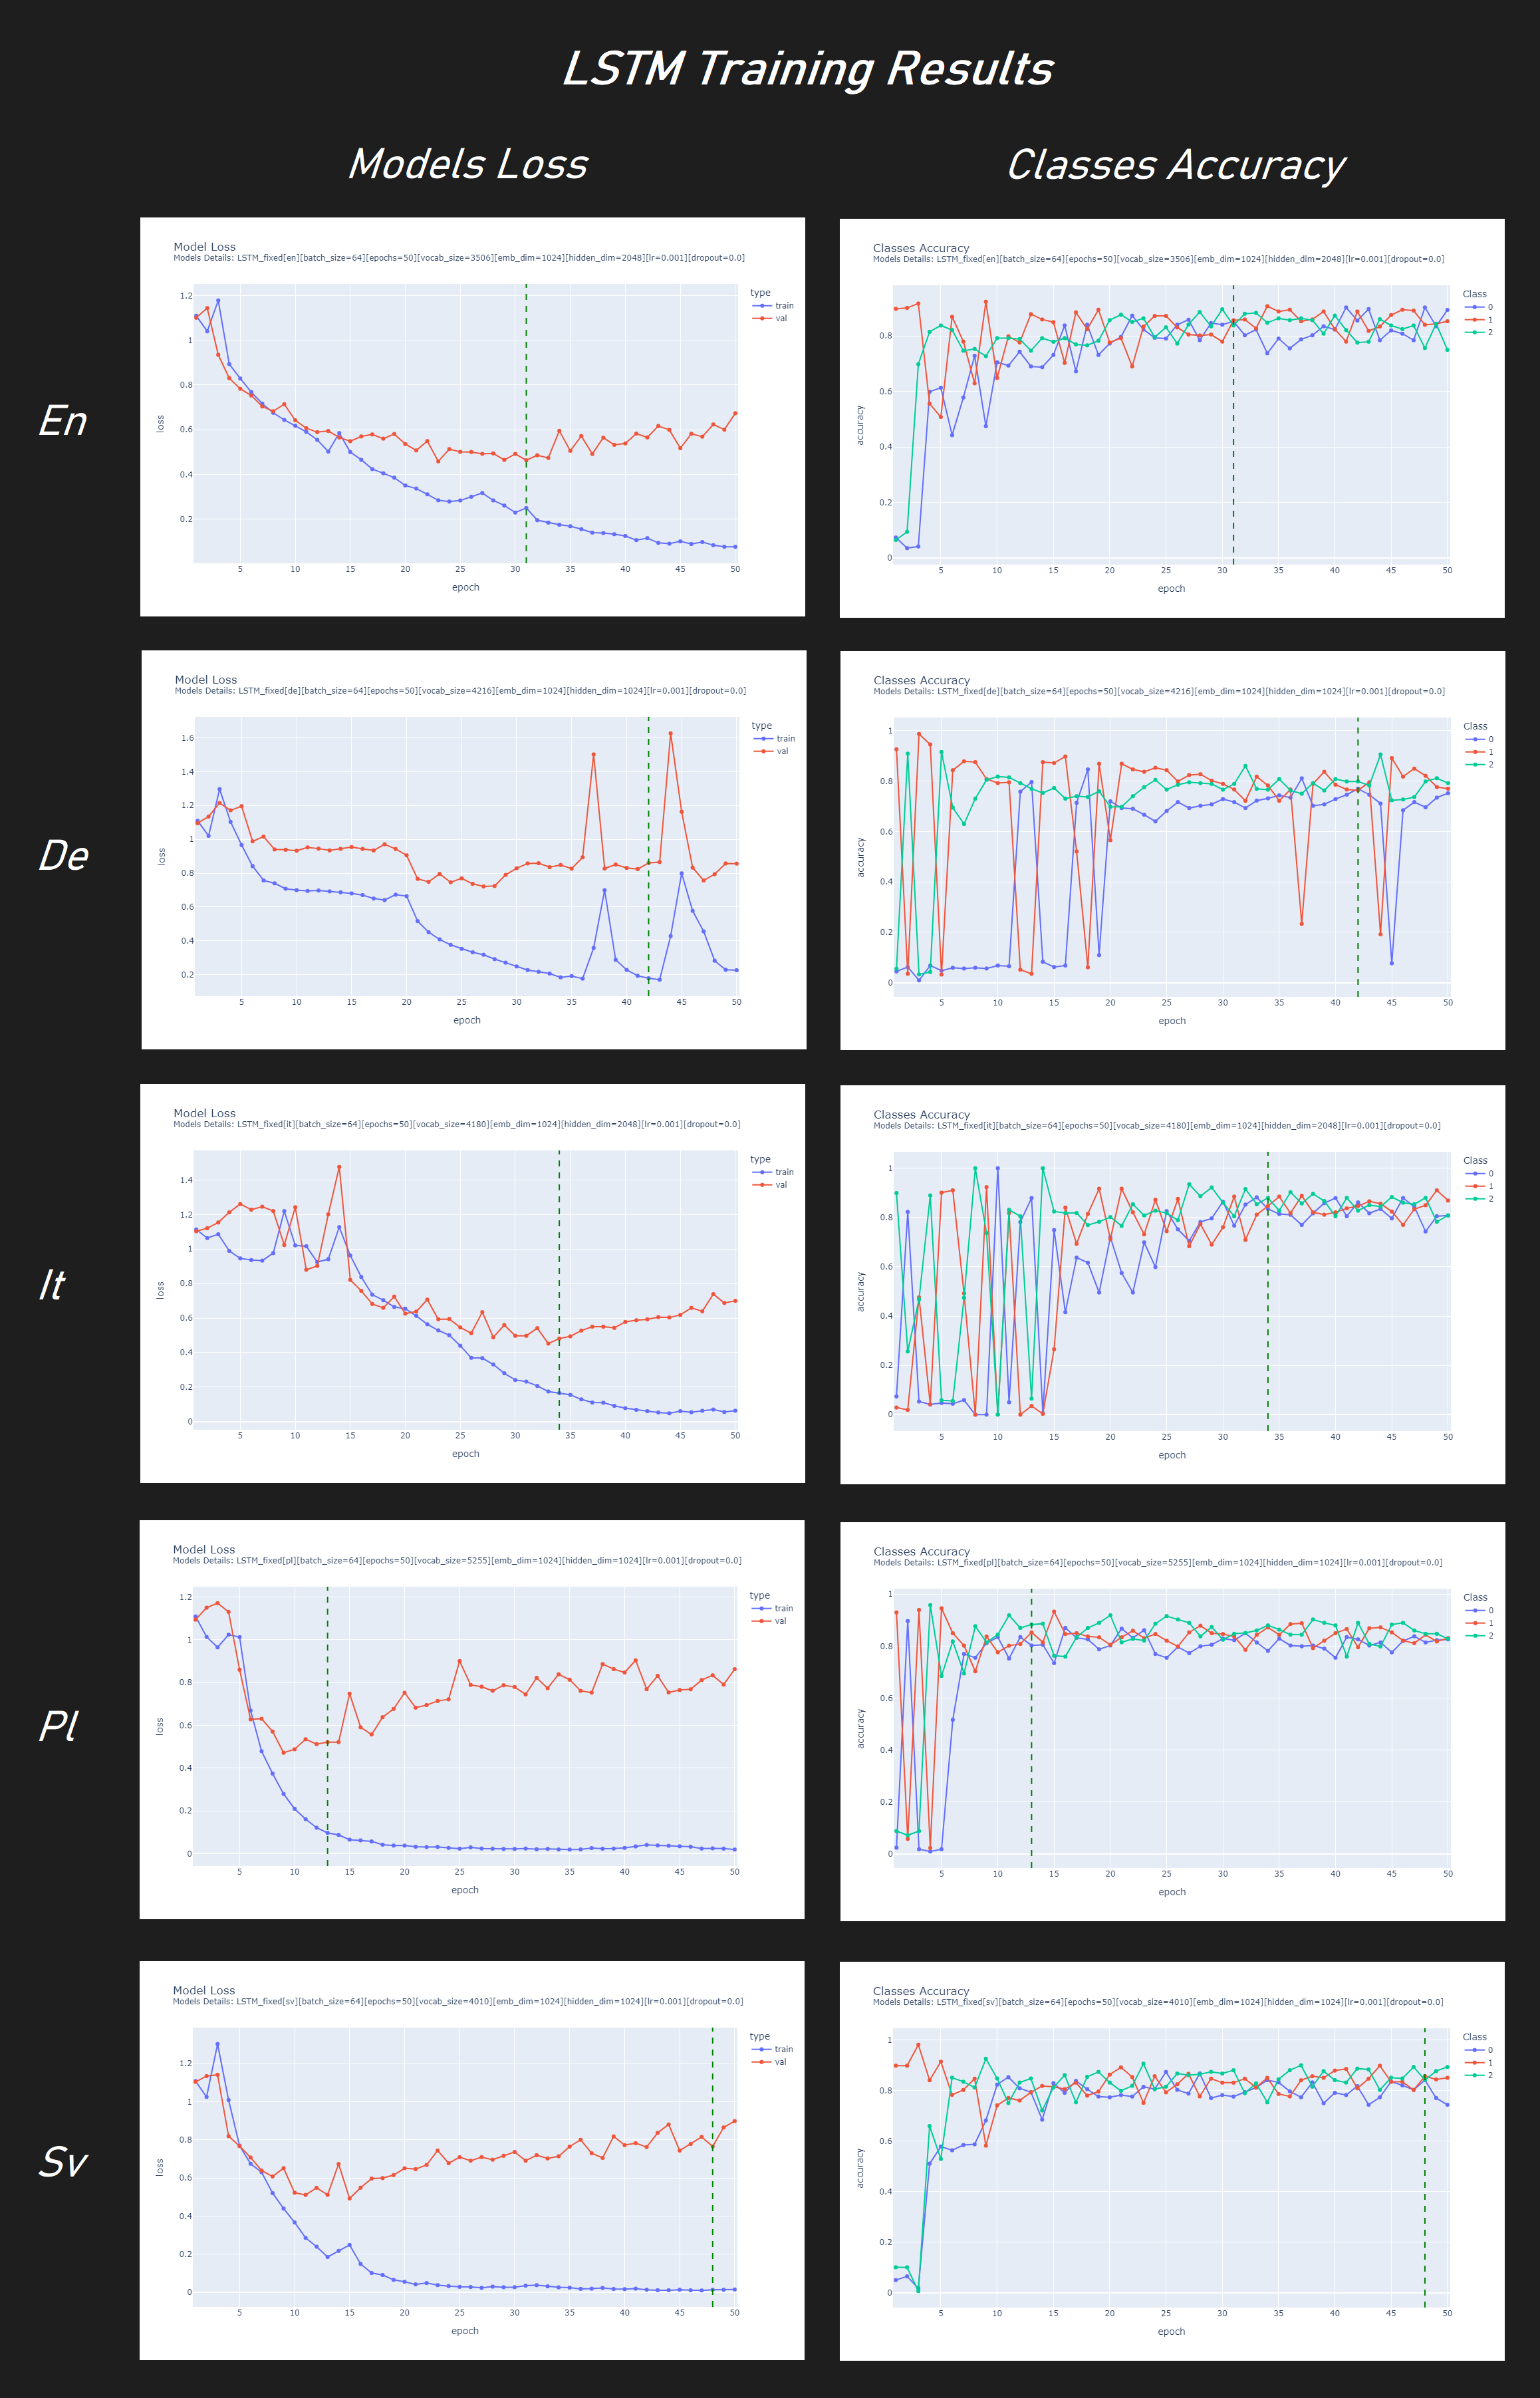
\includegraphics[width=0.995\linewidth]{LSTM_training_results.png}
  }
  \caption{}
  \label{figure:lstm_res}
\end{figure}
\thispagestyle{empty}

\newpage
\pagecolor{resblack}
\begin{figure}[H]
  \vspace*{-1.75cm}
  \makebox[\linewidth]{
    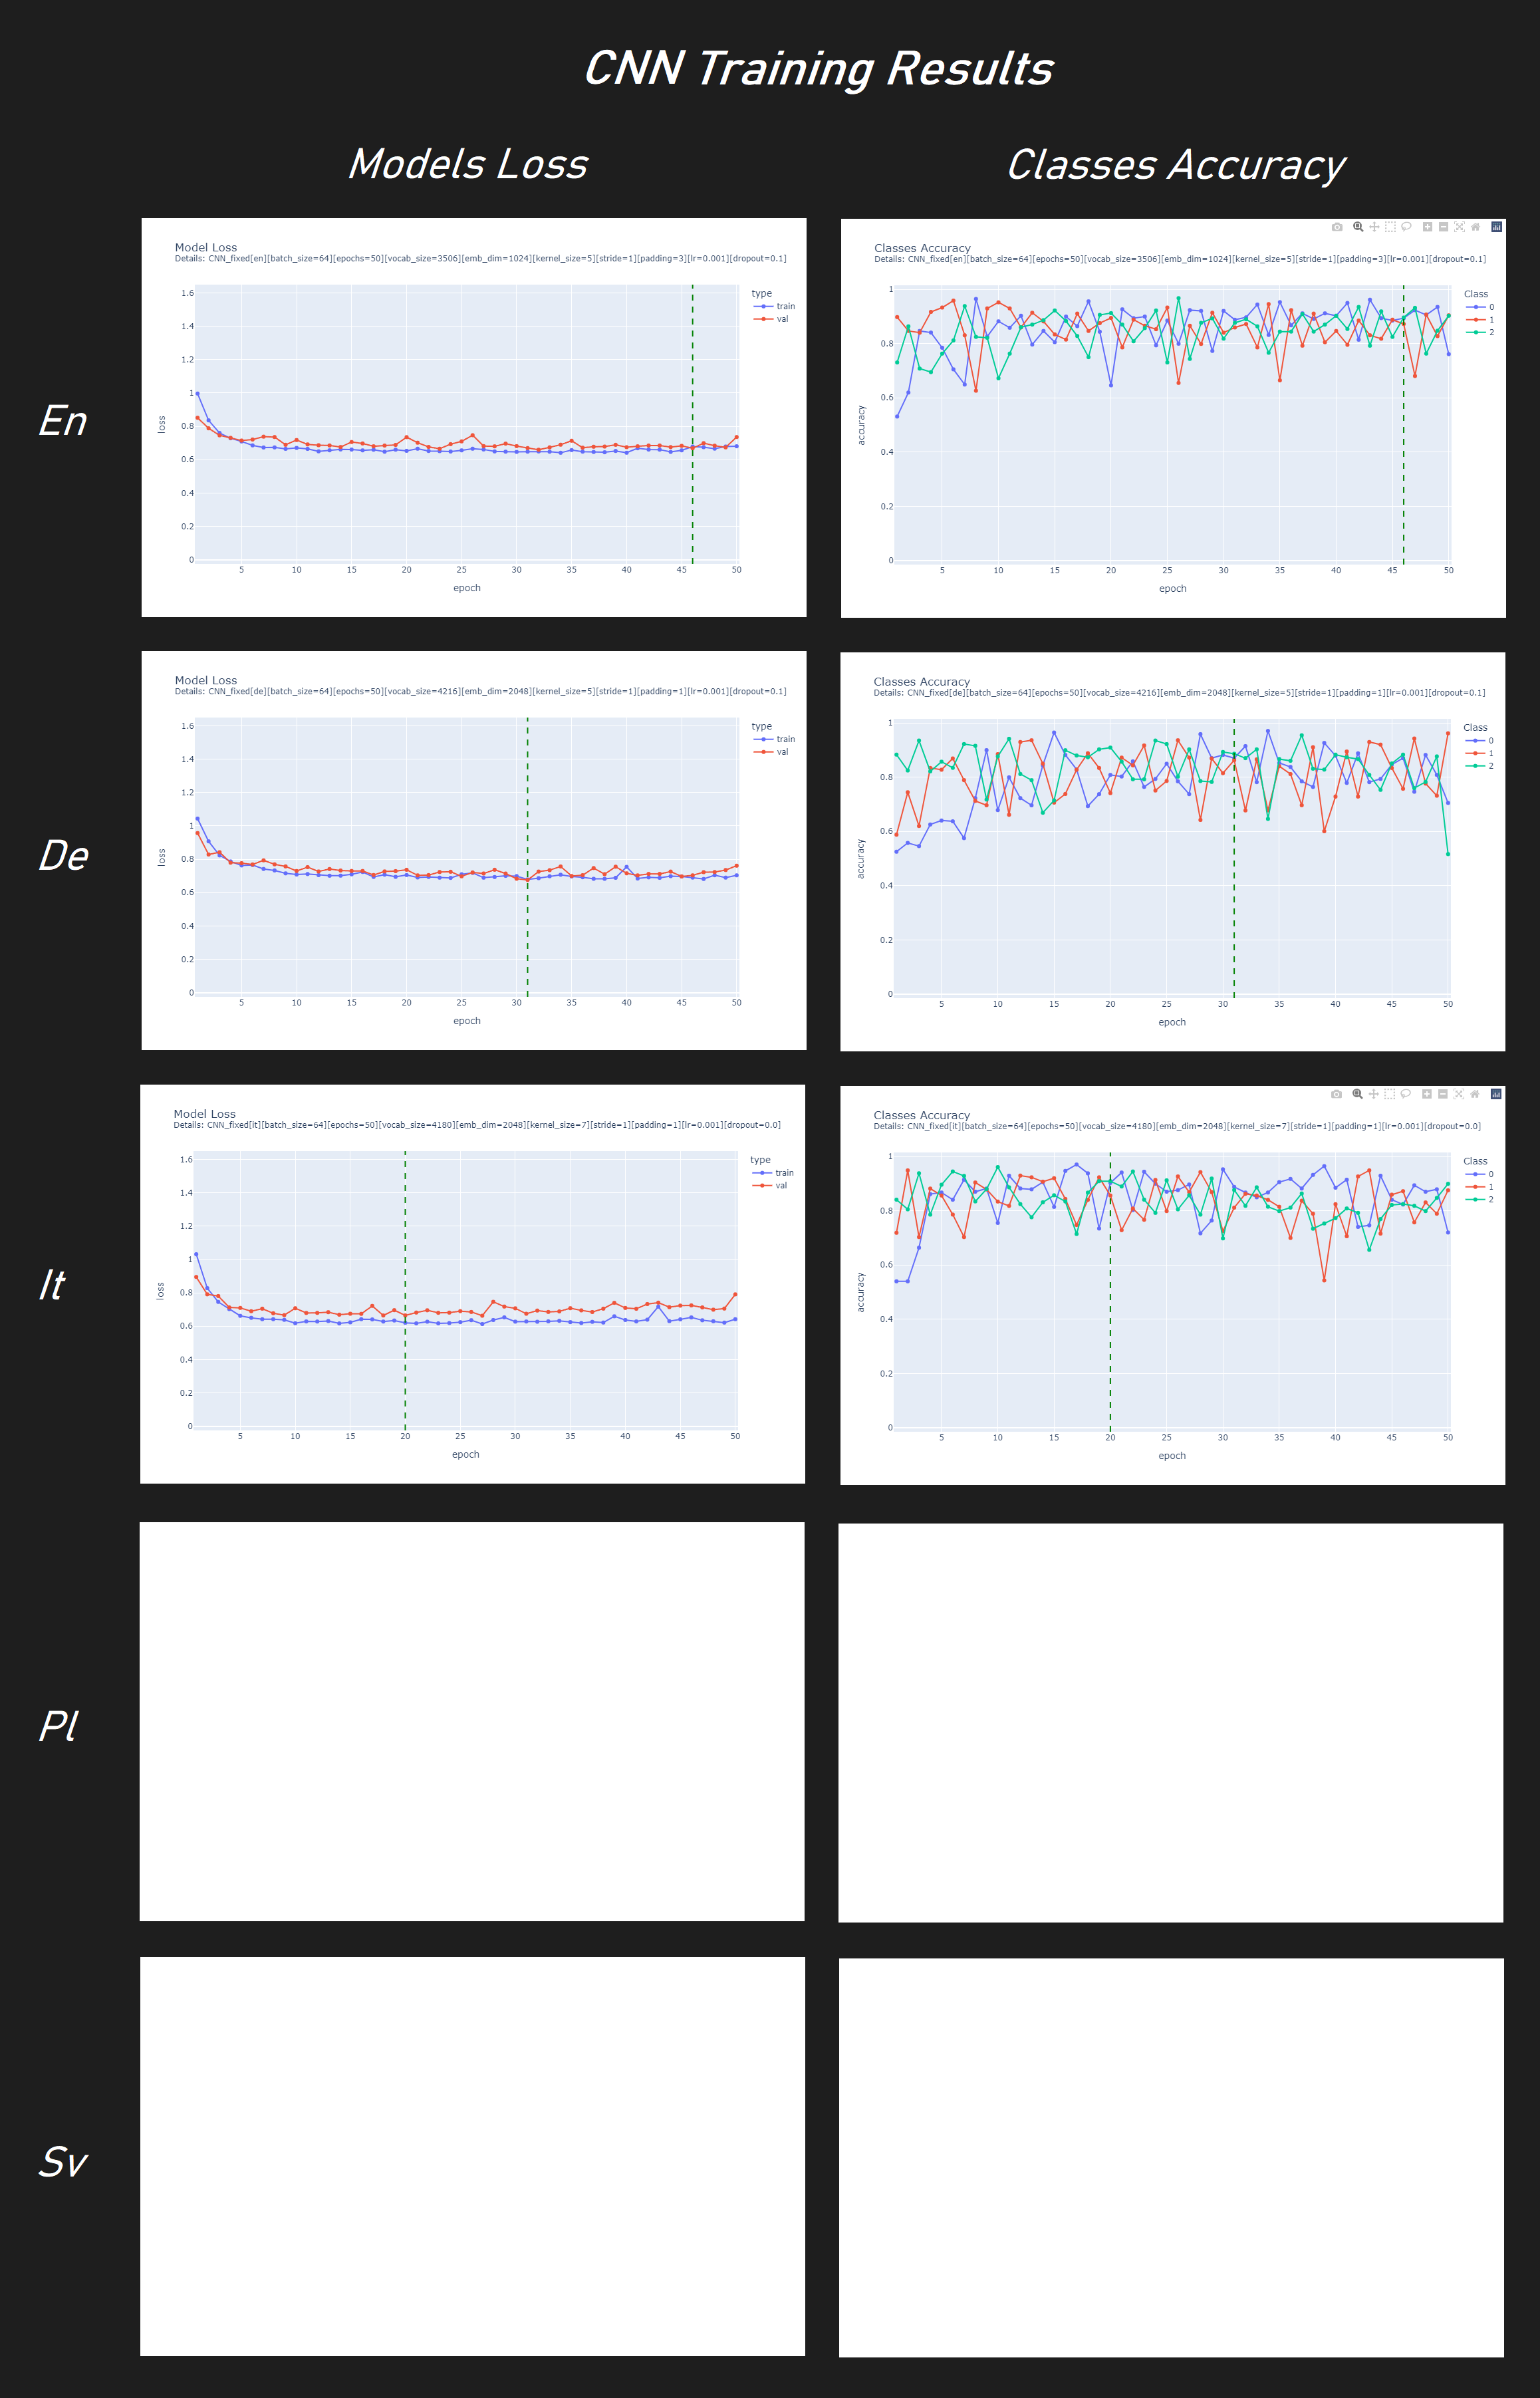
\includegraphics[width=0.995\linewidth]{CNN_training_results.png}
  }
  \caption{}
  \label{figure:cnn_res}
\end{figure}
\thispagestyle{empty} 

%%%%%%%%%%%%%%%%
% BIBLIOGRAPHY %
%%%%%%%%%%%%%%%%

% add bib to TOC
\addcontentsline{toc}{section}{References}

\newpage
\pagecolor{white}
\bibliographystyle{plain}
\bibliography{biblio}

%%%%%%%%%%%%%%%%%%%%%%%%%%%%%%%%%%%%%%%%%%%%%%%%%%%%%%%%%%%%%%%%%%%%%%%%%%%%%%%%%%%%%%%

\end{document}
